\subsection{\texorpdfstring{\textlambda}{lambda}-cubo}
\label{sec:3-lambda-cube}

Prima di discutere l'inferenza di tipo, si vuol descrivere brevemente il \textit{$\lambda$-cubo},
cubo lambda (vedi \textit{Introduction to generalized type systems}, \cite{IntroductionGeneralizedTypeSystems}),
un modello introdotto per classificare i sistemi di tipo applicabili al lambda calcolo,
al fine di comprendere quale sistema il linguaggio \textbf{Funx} implementa.

\noindent In Figura \ref{fig:3-lambda-cube} è possibile osservare come la struttura del cubo abbia all'origine
il \textit{lambda calcolo semplicemente tipato} ($\lambda\mkern-4mu\rightarrow$) e come le tre dimensioni
in cui si sviluppa rappresentino ciascuna un'estensione del sistema:
\begin{itemize}
    \item \textbf{tipi dipendenti} ($\rightarrow$): la definizione dei tipi può dipendere dai valori delle variabili
          (implementati da linguaggi funzionali come \texttt{Agda}, \texttt{Coq} e \texttt{Idris});
    \item \textbf{polimorfismo parametrico} ($\uparrow$): i tipi possono essere polimorfi, generalizzati
          tramite variabili di tipo (presenti nei sistemi adottati da \texttt{ML}, \texttt{OCaml} e \texttt{Haskell});
    \item \textbf{costruttori di tipo} ($\nearrow$): capacità di costruire nuovi tipi a partire da tipi esistenti
          (\texttt{Haskell} ne fa grande uso poiché ogni nuovo tipo,
          dichiarato con la keyword \texttt{data}, è un nuovo costruttore di tipo).
\end{itemize}

\begin{figure}[H]
    \centering
    \usetikzlibrary{3d}
    % messing around for bigger arrow tips
    \usetikzlibrary{arrows.meta}
    \vspace{4mm}
    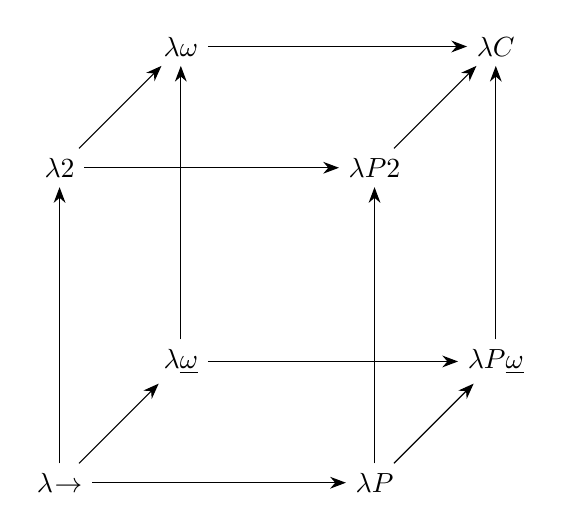
\begin{tikzpicture}[scale=2, >={Stealth[width=1.5mm,length=2mm]}]
        % base, weird xyz coords
        \node (lst) at (0,0,2) {$\lambda\mkern-4mu\rightarrow$};
        \node (lwo) at (0,0,0) {$\lambda\underline{\omega}$};
        \node (lP) at (2,0,2) {$\lambda P$};
        \node (lPwo) at (2,0,0) {$\lambda P\underline{\omega}$};
        % cube hat
        \node (l2) at (0,2,2) {$\lambda2$};
        \node (lo) at (0,2,0) {$\lambda\omega$};
        \node (lP2) at (2,2,2) {$\lambda P2$};
        \node (lC) at (2,2,0) {$\lambda C$}; % woah
        % connect base
        \draw[->] (lst) -- (lwo);
        \draw[->] (lst) -- (lP);
        \draw[->] (lwo) -- (lPwo);
        \draw[->] (lP) -- (lPwo);
        % connect hat
        \draw[->] (l2) -- (lo);
        \draw[->] (l2) -- (lP2);
        \draw[->] (lo) -- (lC);
        \draw[->] (lP2) -- (lC);
        % connect base and hat
        \draw[->] (lst) -- (l2);
        \draw[->] (lwo) -- (lo);
        \draw[->] (lP) -- (lP2);
        \draw[->] (lPwo) -- (lC);
    \end{tikzpicture}
    \caption{\textlambda-cubo}
    \label{fig:3-lambda-cube}
    \vspace{4mm}
\end{figure}

\noindent Senza entrare troppo nei dettagli, in ordine crescente di potenza espressiva:

\begin{itemize}
    \item \textbf{$\lambda\mkern-4mu\rightarrow$} (\textit{lambda calcolo semplicemente tipato}): tipi monomorfi;
    \item \textbf{$\lambda\underline{\omega}$} (\textit{lambda weak omega}): costruttori di tipo;
    \item \textbf{$\lambda2$} (\textit{lambda due, lambda F, lambda calcolo polimorfico}): polimorfismo parametrico;
    \item \textbf{$\lambda P$} (\textit{lambda pi}): tipi dipendenti;
    \item \textbf{$\lambda P\underline{\omega}$} (\textit{lambda pi weak omega}): costruttori di tipo e tipi dipendenti;
    \item \textbf{$\lambda\omega$}: (\textit{lambda omega}): costruttori di tipo e polimorfismo parametrico;
    \item \textbf{$\lambda P2$} (\textit{lambda pi due}): polimorfismo parametrico e tipi dipendenti;
    \item \textbf{$\lambda C$} (\textit{lambda C, calcolo delle costruzioni}): combinazione di tutte le tre estensioni.
\end{itemize}